%导演区
\documentclass[a4paper,11pt,UTF8]{article}%book,report,letter
\usepackage[table]{xcolor}
\usepackage{ctex}
\usepackage{geometry}
\geometry{a4paper,scale=0.8}
\usepackage{amsfonts}
\usepackage{amssymb}
\usepackage{mathrsfs}
\usepackage[arrow,matrix]{xy}
\usepackage{amsmath,amssymb,amscd,bm,bbm,amsthm,mathrsfs}
\usepackage{amsmath,amscd}
\usepackage{amsfonts,amssymb}
\usepackage{xypic}
\usepackage{indentfirst}
\usepackage{diagbox}
\usepackage{graphicx}
\usepackage{subfig}    %% 子图包
\usepackage{float} 
\usepackage{caption}
\captionsetup{labelfont=bf}
\usepackage{zhnumber} % change section number to chinese
%这下面为在latex中插入代码所需环境
\usepackage{CJK}
\usepackage{listings}
\usepackage{xcolor}
\lstset{
	language=Matlab,  %代码语言使用的是matlab
	frame=shadowbox, %把代码用带有阴影的框圈起来
	rulesepcolor=\color{red!20!green!20!blue!20},%代码块边框为淡青色
	keywordstyle=\color{blue!90}\bfseries, %代码关键字的颜色为蓝色,粗体
	commentstyle=\color{red!10!green!70}\textit,    % 设置代码注释的颜色
	showstringspaces=false,%不显示代码字符串中间的空格标记
	numbers=left, % 显示行号
	numberstyle=\tiny,    % 行号字体
	stringstyle=\ttfamily, % 代码字符串的特殊格式
	breaklines=true, %对过长的代码自动换行
	extendedchars=false,  %解决代码跨页时,章节标题,页眉等汉字不显示的问题
	texcl=true}
\def\d{\textup{d}}

\theoremstyle{plain}
\newtheorem{thm}{定理}[section]
\newtheorem{lem}{引理}[section]
\newtheorem{prop}{命题}[section]
\newtheorem{cor}{推论}[section]


\renewcommand{\qedsymbol}{$\square$}
\renewcommand\baselinestretch{1.25}
\renewcommand\thesection{\zhnum{section}}
\renewcommand \thesubsection {\arabic{section}}
%正文区
\begin{document}
	\title{\heiti 课题组组会-练习1}
	\author{王程 }
	\date{\today}
	\maketitle
	
	\section{练习及结果}
	1.\textbf{对带源项的扩散方程$u_t=u_{xx}+\pi^2sin\left(\pi x\right), x\in\left[0,1\right], t\geq 0$ 满足以下初始条件$u\left(x,0\right)=x^2-x$, 及边界条件$u\left(0,t\right)=u\left(1,t\right)=0$}。\\
	~\\
    \indent(1)求该方程的解析稳态解。\\
    \indent(2)使用FHOS引入辅助变量,将上述方程改写成双曲方程组,考虑均匀网格(单元数:8,16,32,64,……),时间离散方法使用显式欧拉格式,空间离散使用DG(P0)+DGP(0)格式,求解稳态解,并与(1) 中的解析解进行对比,测试原始变量$u$和它在$x$方向的导数的空间精度。\\
	\indent(3)将时间离散格式改为BDF1,使用Jacobi迭代法重新对以上方法进行求解,并与显式方法进行对比。\\
	~\\
	\textbf{解:}\\
	\indent(1)方程的解析稳态解为:$u\left(x,t\right)=sin\left(\pi x\right)$。
	\vspace{10pt}\\
	\indent(2)本题仅考虑物理时间达到稳态时的解,时间离散方法使用显式欧拉格式,空间离散使用DG(P0)\\+DG(P0)格式,采用面循环计算RHS,最终得到变形后双曲方程组的稳态解。这里仅展示网格数为8,16,32,64,CFL=0.01的稳态数值解与解析解的比较图,并给出原始变量$u$和它在$x$方向的导数的空间精度比较图。\\
	\newpage
	\textbf{比较$u$稳态数值解和解析解:}
	\begin{figure}[!h]
		\centering
		\subfloat[面循环U8]{
			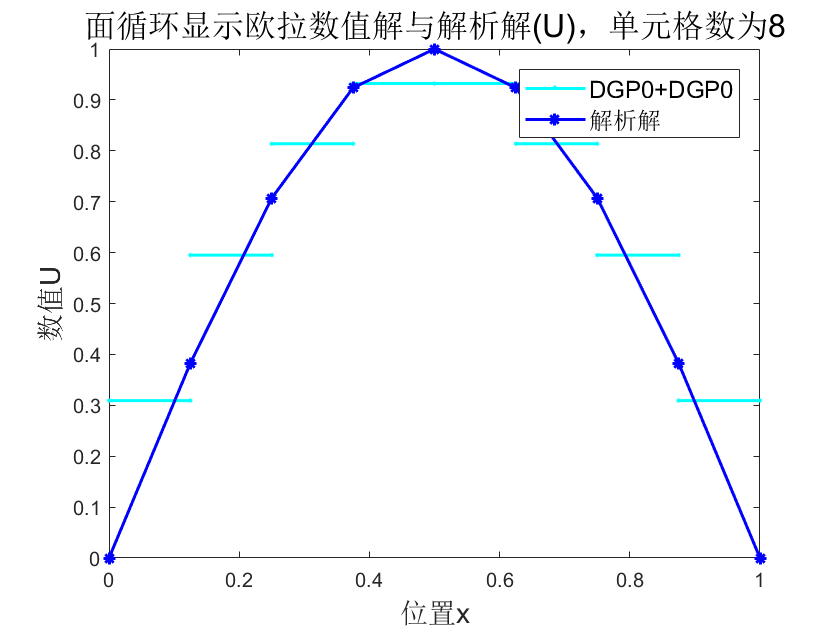
\includegraphics[width=2.5in]{obviousEuler/面循环U8.png} 
		}
	    \hfill
		\subfloat[面循环U16]{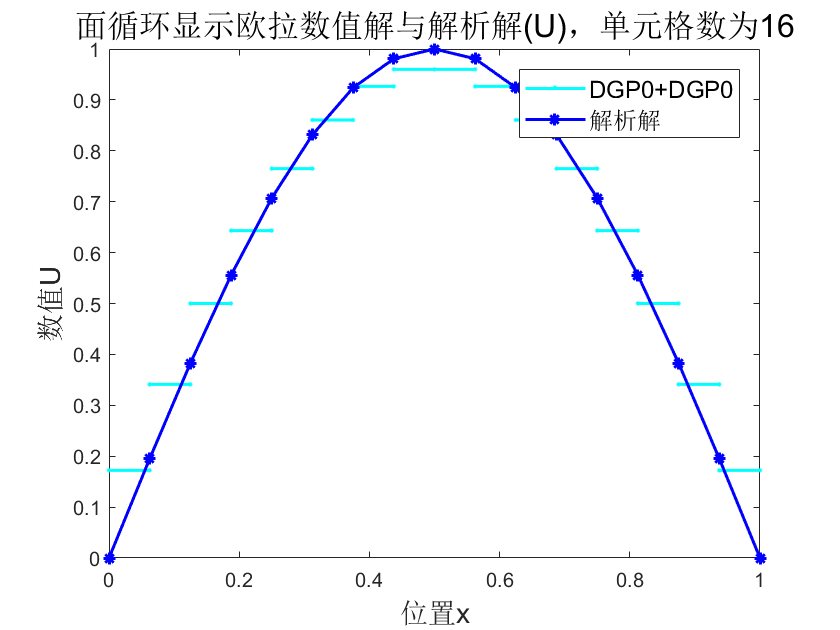
\includegraphics[width=2.5in]{obviousEuler/面循环U16.png} }
		\newline
		\subfloat[面循环U32]{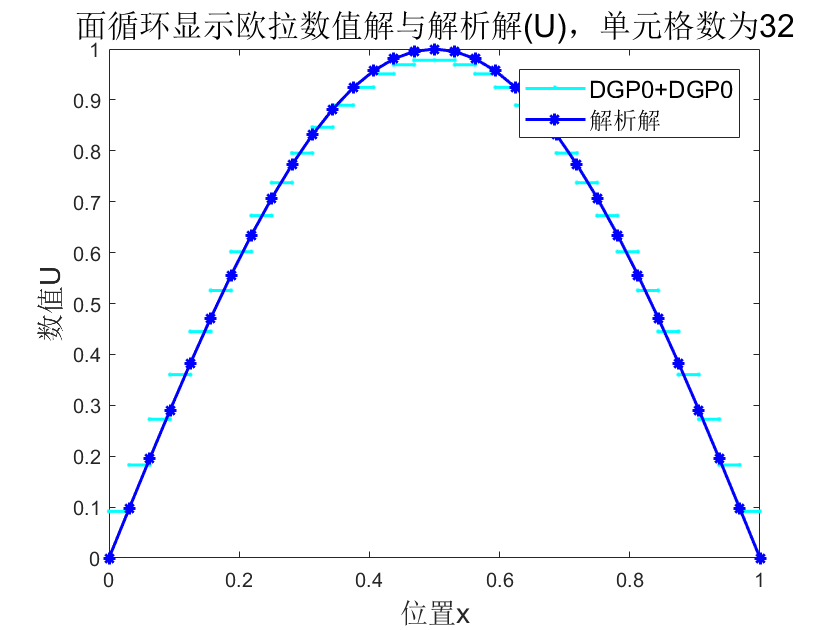
\includegraphics[width=2.5in]{obviousEuler/面循环U32.png} }
		\hfill
		\subfloat[面循环U64]{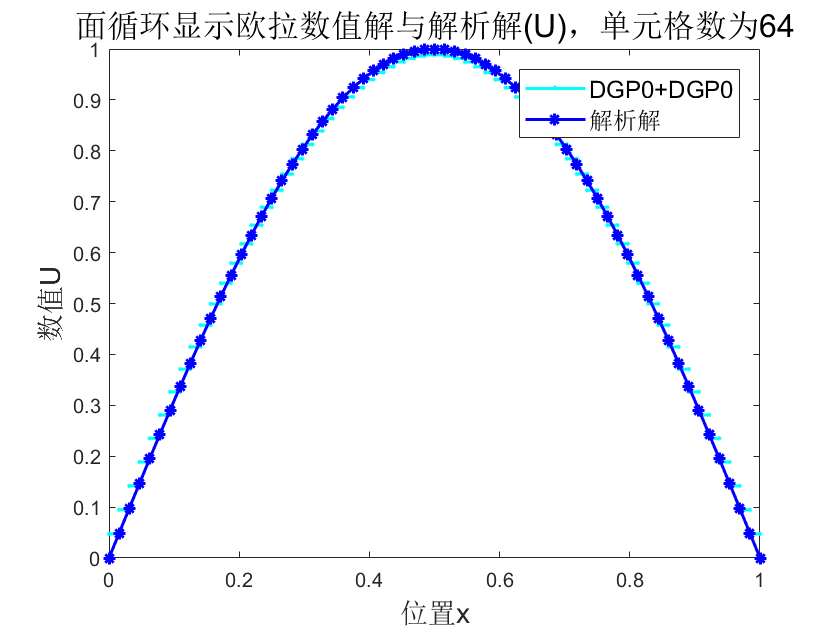
\includegraphics[width=2.5in]{obviousEuler/面循环U64.png} }	
        \caption{显式欧拉面循环求得的$u$稳态解与解析解对比}
	\end{figure}\\

	\indent \textbf{$u$的空间精度:}
\begin{figure}[!h]
	\centering
	\subfloat{
		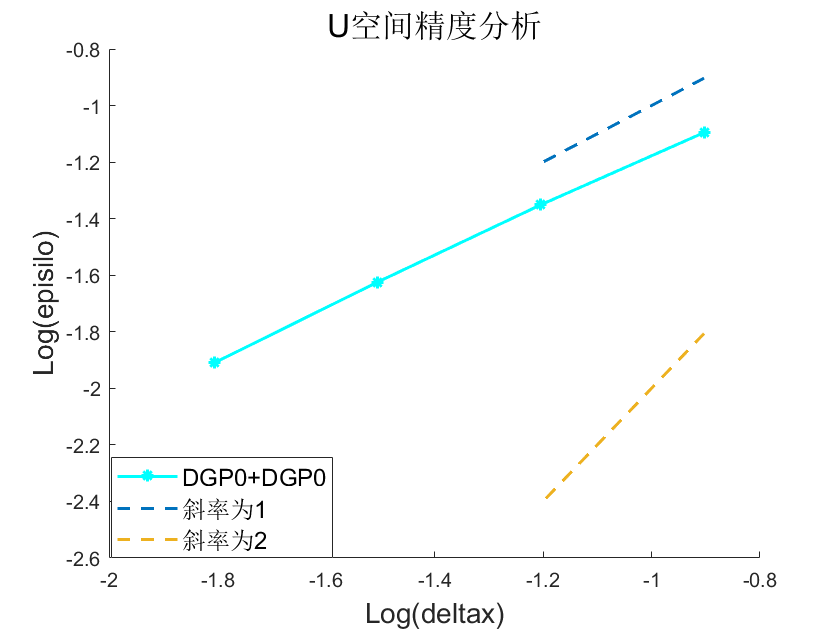
\includegraphics[width=3.5in]{obviousEuler/U空间精度分析.png} 
	}	
	\caption{面循环下$u$空间精度}
\end{figure}\\
\newpage
	\textbf{比较$u_x$稳态数值解和解析解:}
\begin{figure}[!h]
	\centering
	\subfloat[面循环Ux8]{
		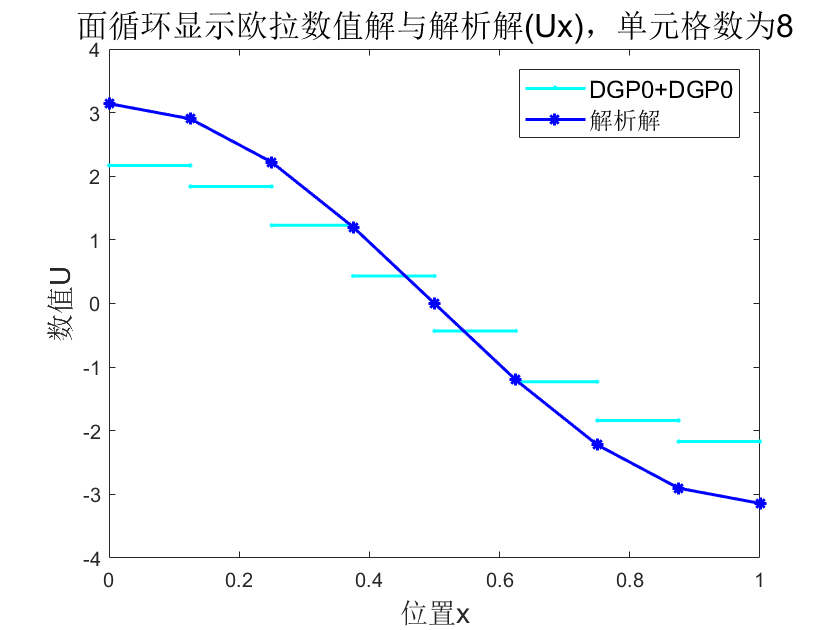
\includegraphics[width=2.5in]{obviousEuler/面循环Ux8.png} 
	}
	\hfill
	\subfloat[面循环Ux16]{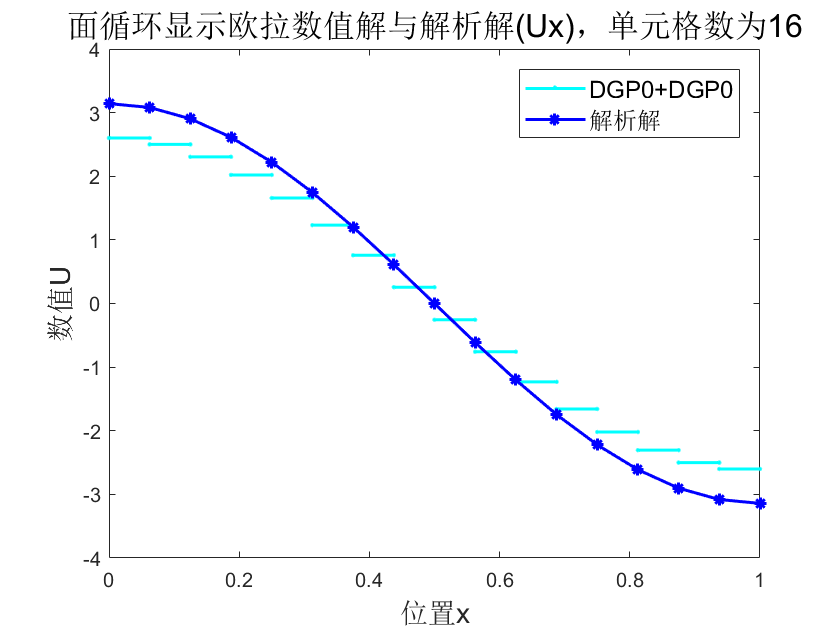
\includegraphics[width=2.5in]{obviousEuler/面循环Ux16.png} }
	\newline
	\subfloat[面循环Ux32]{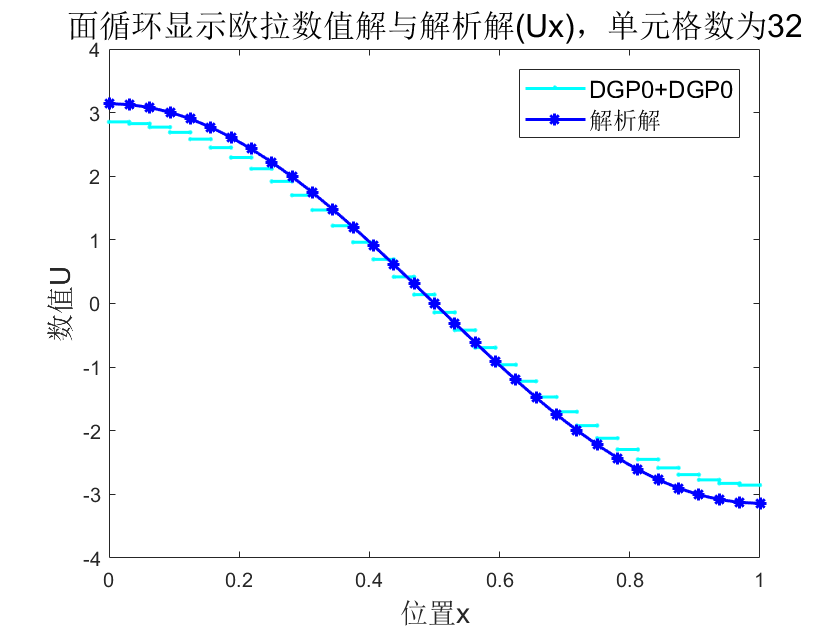
\includegraphics[width=2.5in]{obviousEuler/面循环Ux32.png} }
	\hfill
	\subfloat[面循环Ux64]{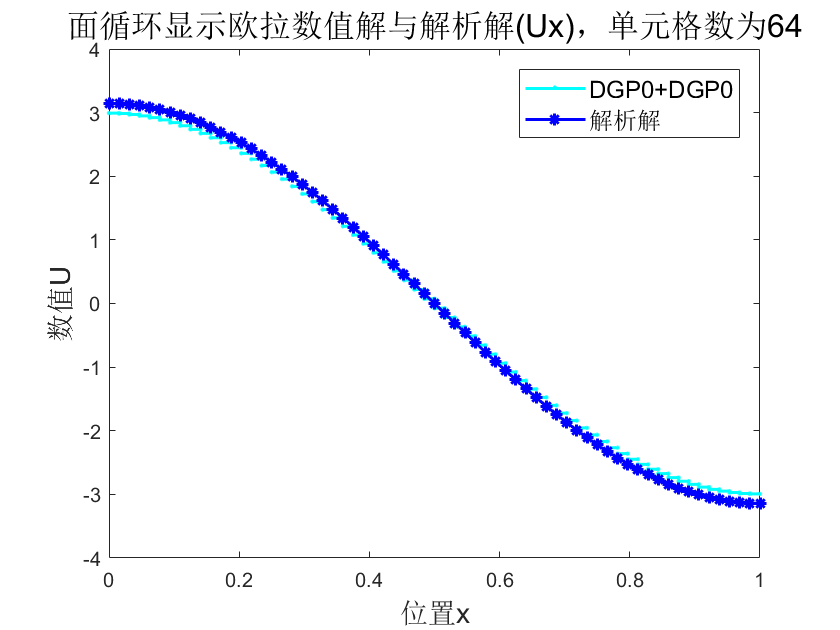
\includegraphics[width=2.5in]{obviousEuler/面循环Ux64.png} }	
	\caption{显式欧拉面循环求得的$u_x$稳态解与解析解对比}
\end{figure}\\


	\indent \textbf{$u_x$的空间精度:}
\begin{figure}[!h]
	\centering

	\subfloat{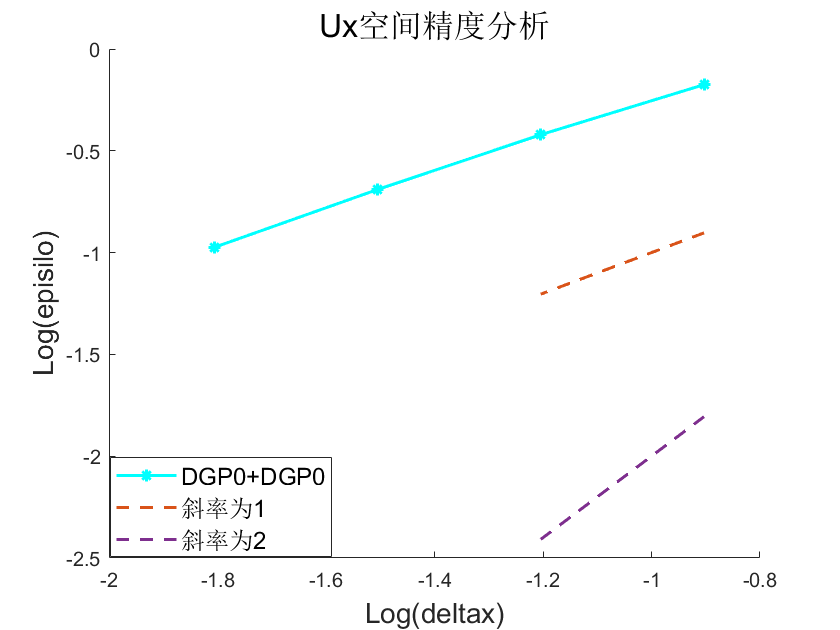
\includegraphics[width=3.5in]{obviousEuler/Ux空间精度分析.png} }
	
	\caption{面循环下$u_x$空间精度}
\end{figure}
\newpage
\indent(3)将时间离散格式改为BDF1,使用Jacobi迭代法重新对该方程的DG(P0)+DG(P0)格式进行求解,采用面循环计算RHS,最终得到变形后双曲方程组的稳态解。这里仅展示网格数为8,16,32,64,CFL=0.01的稳态数值解与解析解的比较图,并给出原始变量$u$和$u_x$的空间精度图。\\
\indent \textbf{比较$u$稳态数值解和解析解:}
\begin{figure}[!h]
	\centering
	\subfloat[面循环U8]{
		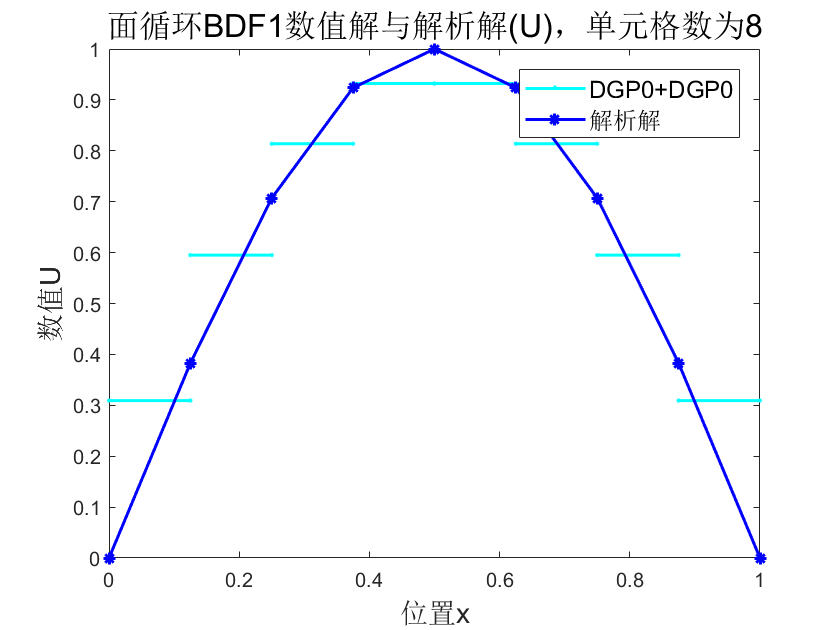
\includegraphics[width=2.5in]{BDF1/BDF1U8.png} 
	}
	\hfill
	\subfloat[面循环U16]{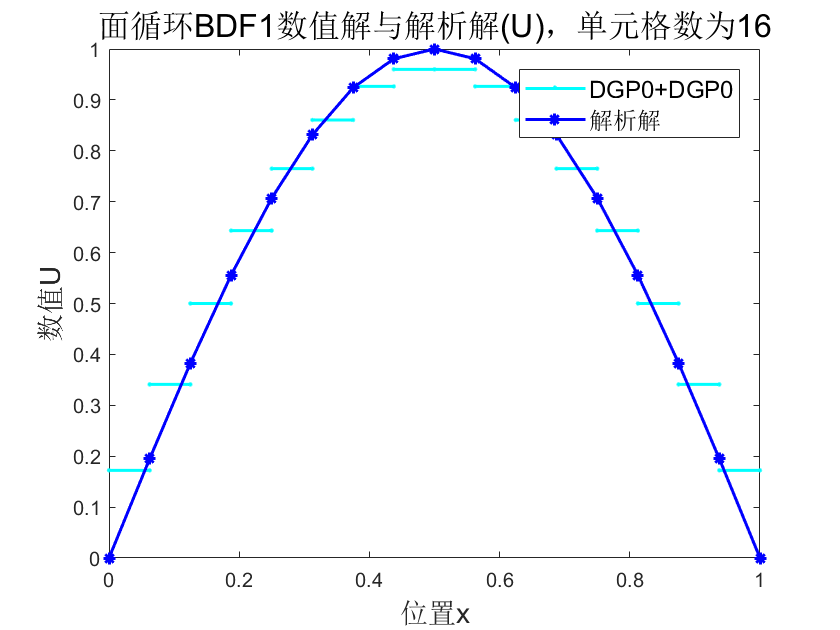
\includegraphics[width=2.5in]{BDF1/BDF1U16.png} }
	\newline
	\subfloat[面循环U32]{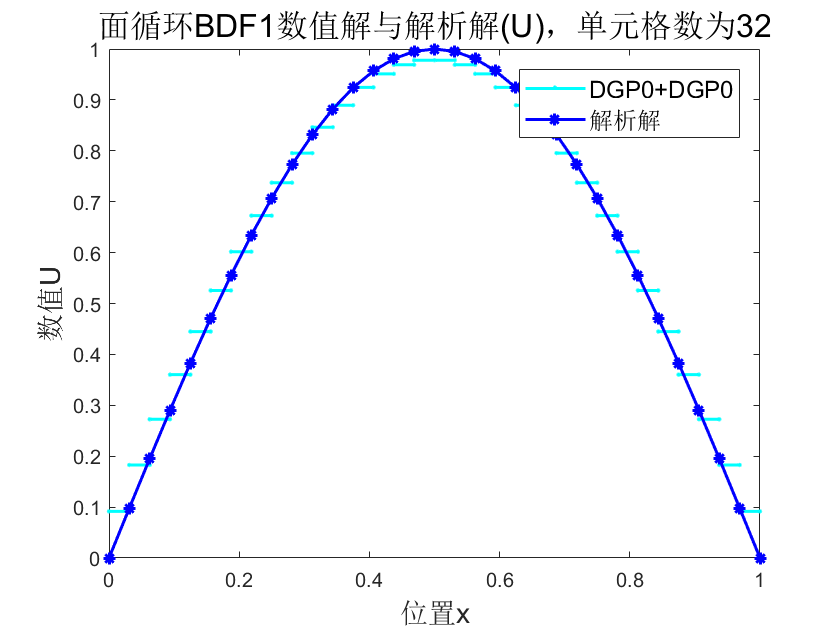
\includegraphics[width=2.5in]{BDF1/BDF1U32.png} }
	\hfill
	\subfloat[面循环U64]{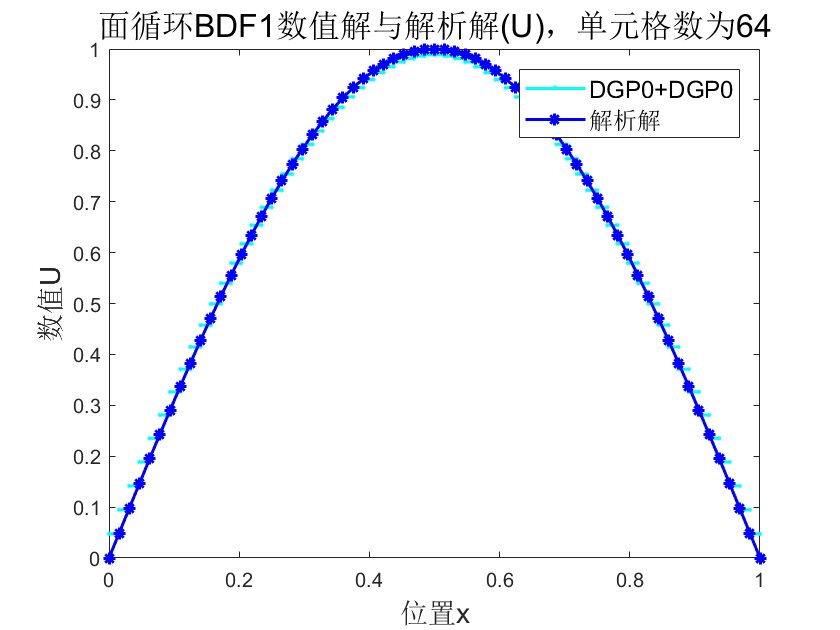
\includegraphics[width=2.5in]{BDF1/BDF1U64.png} }	
	\caption{BDF1面循环求得的$u$稳态解与解析解对比}
\end{figure}\\
\indent \textbf{$u$的空间精度:}
\begin{figure}[!h]
	\centering
	\subfloat{
		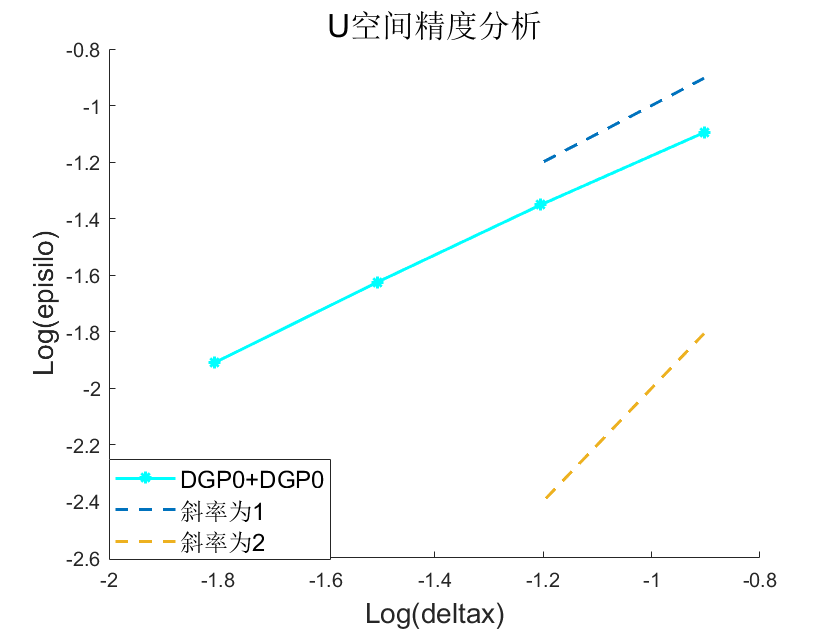
\includegraphics[width=3in]{BDF1/U空间精度分析.png} 
	}	
	\caption{BDF1面循环下$u$空间精度}
\end{figure}
\newpage
\textbf{比较$u_x$稳态数值解和解析解:}
\begin{figure}[!h]
	\centering
	\subfloat[面循环Ux8]{
		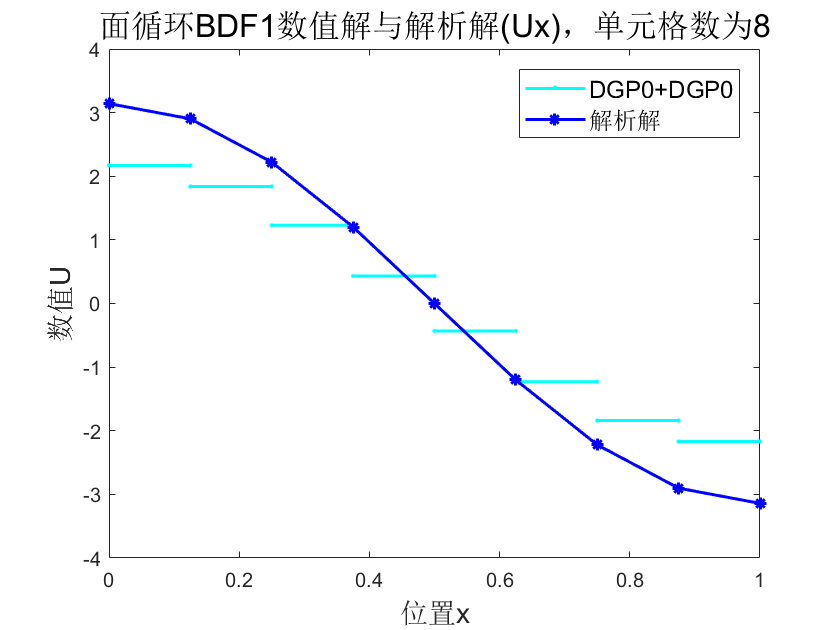
\includegraphics[width=2.5in]{BDF1/BDF1Ux8.png} 
	}
	\hfill
	\subfloat[面循环Ux16]{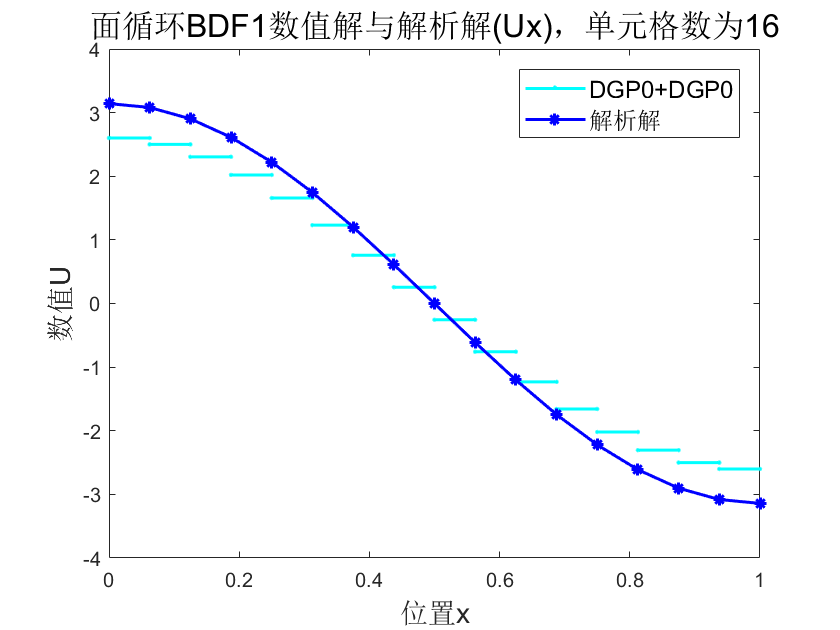
\includegraphics[width=2.5in]{BDF1/BDF1Ux16.png} }
	\newline
	\subfloat[面循环Ux32]{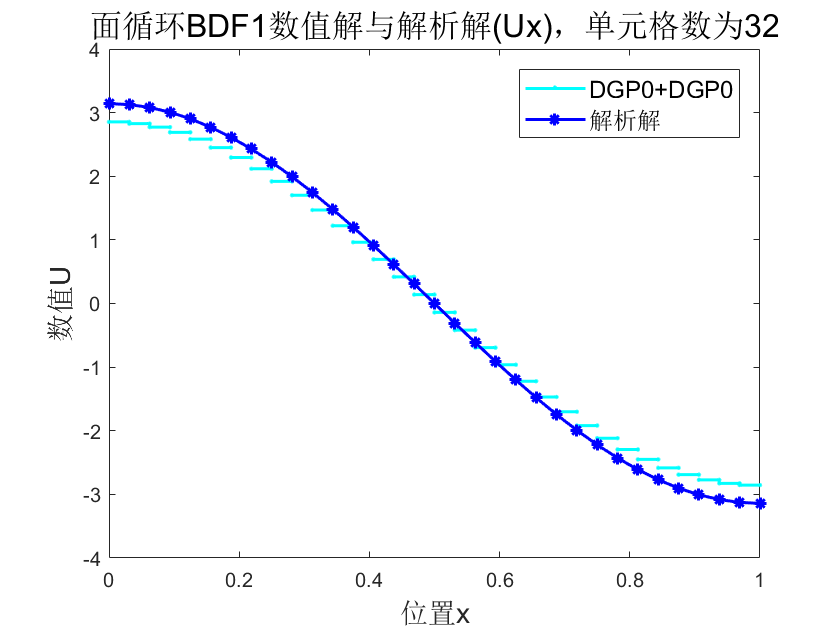
\includegraphics[width=2.5in]{BDF1/BDF1Ux32.png} }
	\hfill
	\subfloat[面循环Ux64]{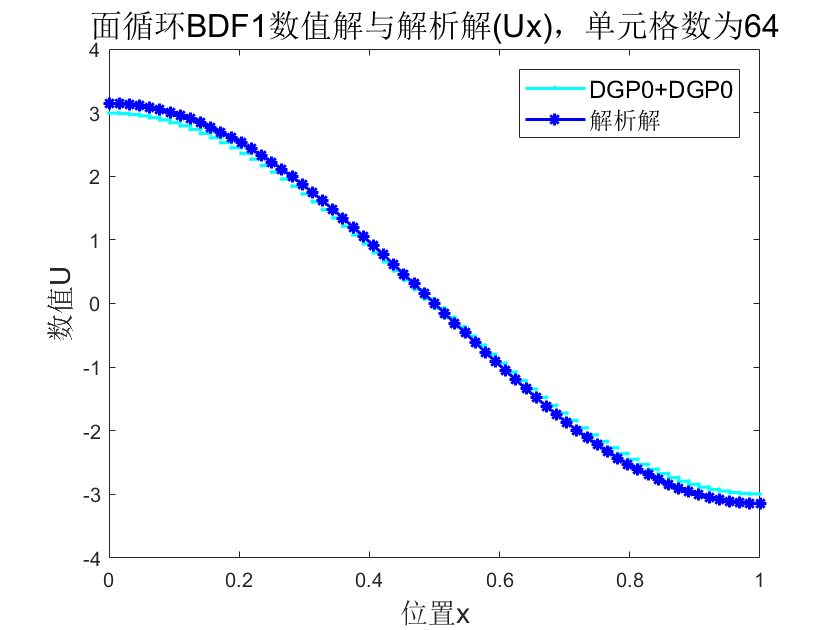
\includegraphics[width=2.5in]{BDF1/BDF1Ux64.png} }	
	\caption{BDF1面循环求得的$u_x$稳态解与解析解对比}
\end{figure}\\


\indent \textbf{$u_x$的空间精度:}
\begin{figure}[!h]
	\centering
	
	\subfloat{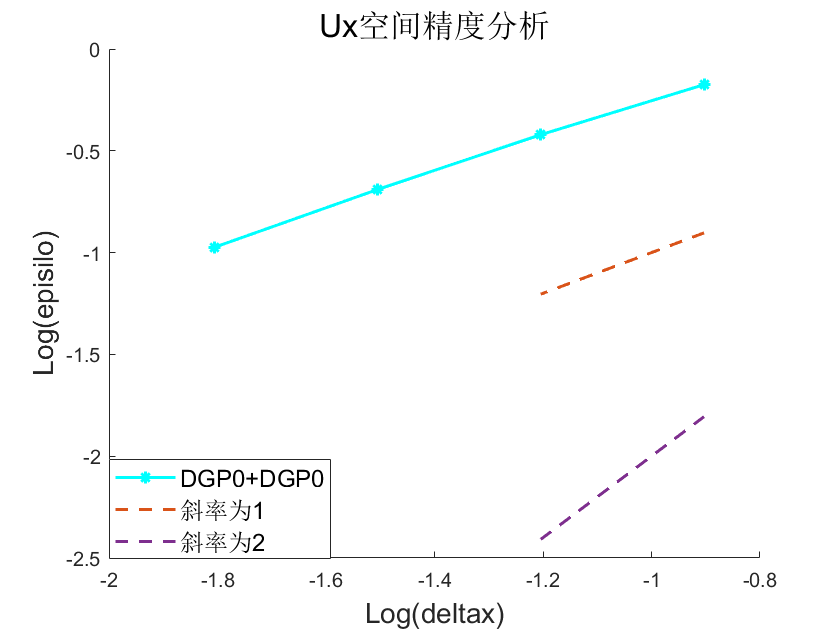
\includegraphics[width=3.5in]{BDF1/Ux空间精度分析.png} }
	
	\caption{BDF1面循环下$u_x$空间精度}
\end{figure}

	\clearpage
	\section{附录(代码)}
	\noindent \textbf{BDF1 main}
	\lstset{language=Matlab}%代码语言使用的是matlab
	\lstset{breaklines}%自动将长的代码行换行排版
	\lstset{extendedchars=false}%解决代码跨页时,章节标题,页眉等汉字不显示的问题
	\begin{lstlisting}
clc
clear all
close all
%% Pre-proceeding
%Some basic paramater
Unit=64;CFL=0.01;endtau=1;endx=1;deltax=endx/Unit;numberx=endx/deltax+1;
tol=10^(-10);
nu=1;Lr=1/(2*pi);Tr=Lr^2/nu;
abslambda=sqrt(nu/Tr);deltatau=CFL*deltax/abslambda;%伪时间变量
B1=1;
C=[B1,0;0,B1/deltax];Mtau=[deltax,0;0,1/deltax];%此为推导出的U=CV中的C
A=[abslambda,0;0,abslambda];
Uexasolution=zeros(2,numberx);
%后处理预设的量
Unumsolution1=zeros(1,2);
Unumsolution2=zeros(2,numberx-1);
%计算空间精度所预设的量
Acc=zeros(3,4);a1=[1/8,1/16,1/32,1/64];a2=[1/8,1/16];
%% Proceeding
%solve the exasolution
x=0;
for k=1:numberx
Uexasolution(1,k)=sin(pi*x);
Uexasolution(2,k)=pi*cos(pi*x);
x=x+deltax;
end
	
[UDGP0plusDGP0,endtau0plus0]=subDGP0plusDGP0(Unit,CFL,endtau);
	
%% Post-proceeding 
%plot the u
%plot the DGP0plusDGP0
figure
x=0*deltax:deltax:1*deltax;
Unumsolution1(1,1)=UDGP0plusDGP0(1,1);Unumsolution1(1,2)=UDGP0plusDGP0(1,1);
plot(x,Unumsolution1,'-c.','linewidth',1.5);hold on
H1=plot(x,Unumsolution1,'-c.','linewidth',1.5);hold on
for i=2:numberx-1
x=(i-1)*deltax:deltax:i*deltax;
Unumsolution1(1,1)=UDGP0plusDGP0(1,i);Unumsolution1(1,2)=UDGP0plusDGP0(1,i);
plot(x,Unumsolution1,'-c.','linewidth',1.5)
end
	
%plot the exact
y=0:deltax:endx;
plot(y,Uexasolution(1,:),'-b*','linewidth',1.5)
H2=plot(y,Uexasolution(1,:),'-b*','linewidth',1.5);hold on
lgd=legend([H1,H2],'DGP0+DGP0','解析解');
lgd.FontSize=12;
xlabel('位置x','fontsize',14)
ylabel('数值U','fontsize',14)
title('面循环BDF1数值解与解析解(U),单元格数为64','fontsize',16)
hold off
	
%plot the ux
%DGP0plusDGP0
figure
x=0*deltax:deltax:1*deltax;
Unumsolution1(1,1)=UDGP0plusDGP0(2,1);Unumsolution1(1,2)=UDGP0plusDGP0(2,1);
plot(x,Unumsolution1,'-c.','linewidth',1.5);hold on
H1=plot(x,Unumsolution1,'-c.','linewidth',1.5);hold on
for i=2:numberx-1
x=(i-1)*deltax:deltax:i*deltax;
Unumsolution1(1,1)=UDGP0plusDGP0(2,i);Unumsolution1(1,2)=UDGP0plusDGP0(2,i);
plot(x,Unumsolution1,'-c.','linewidth',1.5)
end
	
%exact
y=0:deltax:endx;
plot(y,Uexasolution(2,:),'-b*','linewidth',1.5)
H2=plot(y,Uexasolution(2,:),'-b*','linewidth',1.5);hold on
lgd=legend([H1,H2],'DGP0+DGP0','解析解');
lgd.FontSize=12;
xlabel('位置x','fontsize',14)
ylabel('数值U','fontsize',14)
title('面循环BDF1数值解与解析解(Ux),单元格数为64','fontsize',16)
hold off
	
%determine the accuracy of space U
Acc(1,1)=AccuracyU(8,subDGP0plusDGP0(8,CFL,endtau));
Acc(1,2)=AccuracyU(16,subDGP0plusDGP0(16,CFL,endtau));
Acc(1,3)=AccuracyU(32,subDGP0plusDGP0(32,CFL,endtau));
Acc(1,4)=AccuracyU(64,subDGP0plusDGP0(64,CFL,endtau));
	
figure
hold on
plot(log10(a1),log10(Acc(1,:)),'-c*','linewidth',1.5)
H1=plot(log10(a1),log10(Acc(1,:)),'-c*','linewidth',1.5);
	
H2=plot(log10(a2),1*log10(a2),'--','linewidth',1.5);
plot(log10(a2),2*log10(a2),'--','linewidth',1.5)
H3=plot(log10(a2),2*log10(a2),'--','linewidth',1.5);
lgd=legend([H1,H2,H3],'DGP0+DGP0','斜率为1','斜率为2');
lgd.FontSize=12;
xlabel('Log(deltax)','fontsize',14)
ylabel('Log(episilo)','fontsize',14)
title('U空间精度分析','fontsize',16)
	
%determine the accuracy of space Ux
%DGP0
Acc(1,1)=AccuracyUx(8,subDGP0plusDGP0(8,CFL,endtau));
Acc(1,2)=AccuracyUx(16,subDGP0plusDGP0(16,CFL,endtau));
Acc(1,3)=AccuracyUx(32,subDGP0plusDGP0(32,CFL,endtau));
Acc(1,4)=AccuracyUx(64,subDGP0plusDGP0(64,CFL,endtau));
	
figure
hold on
plot(log10(a1),log10(Acc(1,:)),'-c*','linewidth',1.5)
H1=plot(log10(a1),log10(Acc(1,:)),'-c*','linewidth',1.5);
	
plot(log10(a2),1*log10(a2),'--','linewidth',1.5)
H2=plot(log10(a2),1*log10(a2),'--','linewidth',1.5);
plot(log10(a2),2*log10(a2),'--','linewidth',1.5)
H3=plot(log10(a2),2*log10(a2),'--','linewidth',1.5);
lgd=legend([H1,H2,H3],'DGP0+DGP0','斜率为1','斜率为2');
lgd.FontSize=12;
xlabel('Log(deltax)','fontsize',14)
ylabel('Log(episilo)','fontsize',14)
title('Ux空间精度分析','fontsize',16)
	\end{lstlisting}
\newpage
\noindent \textbf{BDF1 function DG(P0)+DG(P0)}
\begin{lstlisting}
function [Unumsolution,n]=subDGP0plusDGP0(Unit,CFL,endtau)
%Some basic paramater
endx=1;deltax=endx/Unit;numberx=endx/deltax+1;
tol=10^(-10);
nu=1;Lr=1/(2*pi);Tr=Lr^2/nu;
abslambda=sqrt(nu/Tr);deltatau=CFL*deltax/abslambda;%伪时间变量
B1=1;
C=[B1,0;0,B1/deltax];Mtau=[deltax,0;0,1/deltax];%此为推导出的U=CV中的C
A=[abslambda,0;0,abslambda];
R=zeros(2*Unit,1);
Rd=zeros(2,numberx-1);
Rb=zeros(2,numberx-1);
Fn=zeros(2,numberx);

%构建LHS
%Mtau/deltatau
LHS1=sparse(1:2:2*Unit-1,1:2:2*Unit-1,deltax/deltatau,2*Unit,2*Unit);
LHS1=LHS1+sparse(2:2:2*Unit,2:2:2*Unit,1/(deltax*deltatau),2*Unit,2*Unit);
%Rdomain
LHS2=-sparse(2:2:2*Unit,2:2:2*Unit,-1/(Tr*deltax),2*Unit,2*Unit);
%Rboundary
LHS3=zeros(2*Unit,2*Unit);
for iface=2:numberx-1
ieL=iface-1;
ieR=iface;
%diag
LHS3(2*ieL-1:2*ieL,2*ieL-1:2*ieL)=LHS3(2*ieL-1:2*ieL,2*ieL-1:2*ieL)+C'*[abslambda/2,-nu/(2*deltax);-1/(2*Tr),abslambda/(2*deltax)];
LHS3(2*ieR-1:2*ieR,2*ieR-1:2*ieR)=LHS3(2*ieR-1:2*ieR,2*ieR-1:2*ieR)-C'*[-abslambda/2,-nu/(2*deltax);-1/(2*Tr),-abslambda/(2*deltax)];
%upper
LHS3(2*ieL-1:2*ieL,2*ieR-1:2*ieR)=LHS3(2*ieL-1:2*ieL,2*ieR-1:2*ieR)+C'*[-abslambda/2,-nu/(2*deltax);-1/(2*Tr),-abslambda/(2*deltax)];
%lower
LHS3(2*ieR-1:2*ieR,2*ieL-1:2*ieL)=LHS3(2*ieR-1:2*ieR,2*ieL-1:2*ieL)-C'*[abslambda/2,-nu/(2*deltax);-1/(2*Tr),abslambda/(2*deltax)];
end
LHS3(2*1-1:2*1,2*1-1:2*1)=LHS3(2*1-1:2*1,2*1-1:2*1)-C'*([abslambda/2,-nu/2;-1/(2*Tr),abslambda/2]*[0,0;0,1]+[-abslambda/2,-nu/2;-1/(2*Tr),-abslambda/2])*C;
LHS3(2*(numberx-1)-1:2*(numberx-1),2*(numberx-1)-1:2*(numberx-1))=LHS3(2*(numberx-1)-1:2*(numberx-1),2*(numberx-1)-1:2*(numberx-1))+C'*([abslambda/2,-nu/2;-1/(2*Tr),abslambda/2]+[-abslambda/2,-nu/2;-1/(2*Tr),-abslambda/2]*[0,0;0,1])*C;

LHS=LHS1+LHS2+LHS3;

%取出我们所需要的D
D=zeros(2*Unit,2*Unit);
for iface=2:numberx
ieL=iface-1;
D(2*ieL-1:2*ieL,2*ieL-1:2*ieL)=LHS(2*ieL-1:2*ieL,2*ieL-1:2*ieL);
end
%为循环所预设的一些量
Ucurrent=zeros(2,numberx-1);
Unext=zeros(2*Unit,1);
%initial  condition set up
x=0;
for k=1:numberx-1
Ucurrent(1,k)=(x+deltax/2)^2-(x+deltax/2);
Ucurrent(2,k)=(2*(x+deltax/2)-1)*deltax;
x=x+deltax;
end

%Rdomain
x=0;
for k=1:numberx-1
Rd(1,k)=pi*(cos(pi*x)-cos(pi*(x+deltax)));
Rd(2,k)=-Ucurrent(2,k)/(Tr*deltax);
x=x+deltax;
end
%Rboundary
for iface=2:numberx-1
ieL=iface-1;
ieR=iface;
Fn(:,iface)=0.5*([-nu*Ucurrent(2,ieL)/deltax;-Ucurrent(1,ieL)/Tr]+[-nu*Ucurrent(2,ieR)/deltax;-Ucurrent(1,ieR)/Tr])-0.5*A*([Ucurrent(1,ieR);Ucurrent(2,ieR)/deltax]-[Ucurrent(1,ieL);Ucurrent(2,ieL)/deltax]);
Rb(:,ieL)=Rb(:,ieL)-C'*Fn(:,iface);
Rb(:,ieR)=Rb(:,ieR)+C'*Fn(:,iface);
end
Fn(:,1)=0.5*([-nu*Ucurrent(2,1)/deltax;0]+[-nu*Ucurrent(2,1)/deltax;-Ucurrent(1,1)/Tr])-0.5*A*([Ucurrent(1,1);Ucurrent(2,1)/deltax]-[0;Ucurrent(2,1)/deltax]);
Fn(:,numberx)=0.5*([-nu*Ucurrent(2,numberx-1)/deltax;-Ucurrent(1,numberx-1)/Tr]+[-nu*Ucurrent(2,numberx-1)/deltax;0])-0.5*A*([0;Ucurrent(2,numberx-1)/deltax]-[Ucurrent(1,numberx-1);Ucurrent(2,numberx-1)/deltax]);
Rb(:,1)=Rb(:,1)+C'*Fn(:,1);
Rb(:,numberx-1)=Rb(:,numberx-1)-C'*Fn(:,numberx);

%R组装
for k=1:numberx-1
R(2*k-1:2*k,1)=Rd(:,k)+Rb(:,k);
end
%进行必要的向量等价转变
for k=1:numberx-1
Unext(2*k-1:2*k,1)=Ucurrent(:,k);
end
%循环迭代
for n=deltatau:deltatau:endtau
X=D\R;
if max(X)<tol
break
end
Unext=Unext+X;
Rd=zeros(2,numberx-1);
Rb=zeros(2,numberx-1);    
for k=1:numberx-1
Ucurrent(:,k)=Unext(2*k-1:2*k,1);
end
%Rdomain
x=0;
for k=1:numberx-1
Rd(1,k)=pi*(cos(pi*x)-cos(pi*(x+deltax)));
Rd(2,k)=-Ucurrent(2,k)/(Tr*deltax);
x=x+deltax;
end
%Rboundary
for iface=2:numberx-1
ieL=iface-1;
ieR=iface;
Fn(:,iface)=0.5*([-nu*Ucurrent(2,ieL)/deltax;-Ucurrent(1,ieL)/Tr]+[-nu*Ucurrent(2,ieR)/deltax;-Ucurrent(1,ieR)/Tr])-0.5*A*([Ucurrent(1,ieR);Ucurrent(2,ieR)/deltax]-[Ucurrent(1,ieL);Ucurrent(2,ieL)/deltax]);
Rb(:,ieL)=Rb(:,ieL)-C'*Fn(:,iface);
Rb(:,ieR)=Rb(:,ieR)+C'*Fn(:,iface);
end
Fn(:,1)=0.5*([-nu*Ucurrent(2,1)/deltax;0]+[-nu*Ucurrent(2,1)/deltax;-Ucurrent(1,1)/Tr])-0.5*A*([Ucurrent(1,1);Ucurrent(2,1)/deltax]-[0;Ucurrent(2,1)/deltax]);
Fn(:,numberx)=0.5*([-nu*Ucurrent(2,numberx-1)/deltax;-Ucurrent(1,numberx-1)/Tr]+[-nu*Ucurrent(2,numberx-1)/deltax;0])-0.5*A*([0;Ucurrent(2,numberx-1)/deltax]-[Ucurrent(1,numberx-1);Ucurrent(2,numberx-1)/deltax]);
Rb(:,1)=Rb(:,1)+C'*Fn(:,1);
Rb(:,numberx-1)=Rb(:,numberx-1)-C'*Fn(:,numberx);

%R组装
for k=1:numberx-1
R(2*k-1:2*k,1)=Rd(:,k)+Rb(:,k);
end

for k=1:numberx-1
Unext(2*k-1:2*k,1)=Ucurrent(:,k);
end
end
Unumsolution(1,:)=Ucurrent(1,:);Unumsolution(2,:)=Ucurrent(2,:)/deltax;
end

\end{lstlisting}
\newpage
\noindent \textbf{$u$空间精度分析}
\begin{lstlisting}
function A=AccuracyU(Unit,Unumsolution)
%% Pre-processing
deltx=1/Unit;endx=1;
numberx=endx/deltx+1;
%calculate the accuracy of space DGp0+DGP0
I1=0;t=[-1/sqrt(5),0,1/sqrt(5)];W=[5/9,8/9,5/9];
k=1;%determine the correctness of the program
for x=0:deltx:endx-deltx
for i=1:3
xi=deltx/2*t(i)+0.5*(2*x+deltx);
for m=1:numberx-1
if xi>(m-1)*deltx&&xi<m*deltx
fi=(sin(pi*xi)-Unumsolution(1,m))^2;k=k+1;
end
end
I1=I1+W(i)*fi;
end
end
I1=I1*0.5*deltx;
A=sqrt(I1);
end
\end{lstlisting}
\newpage
\noindent \textbf{$u_x$空间精度分析}
\begin{lstlisting}
function A1=AccuracyUx(Unit,Unumsolution)
%% Pre-processing
deltx=1/Unit;endx=1;
numberx=endx/deltx+1;
%calculate the accuracy of space
I2=0;t=[-1/sqrt(5),0,1/sqrt(5)];W=[5/9,8/9,5/9];
k=1;%determine the correctness of the program
for x=0:deltx:endx-deltx
for i=1:3
xi=deltx/2*t(i)+0.5*(2*x+deltx);
for m=1:numberx-1
if xi>(m-1)*deltx&&xi<m*deltx
fi=(pi*cos(pi*xi)-Unumsolution(2,m))^2;k=k+1;
end
end
I2=I2+W(i)*fi;
end
end
I2=I2*0.5*deltx;
A1=sqrt(I2);
end
	
\end{lstlisting}



\end{document}